\documentclass{llncs}

\usepackage{amsmath}
\usepackage{amssymb}
\usepackage{graphicx}
\usepackage{enumerate}
\usepackage{url}

\newcommand{\tup}[1]{\langle #1 \rangle}
\newcommand{\vvec}[1]{\mathbf{#1}}
\newcommand{\join}{\bowtie}
\newcommand{\R}{\mathcal{R}}
\newcommand{\Q}{\mathcal{Q}}
\newcommand{\qrule}{:\!\!-}
\newcommand{\mcdsat}{\textsc{McdSat}}
\newcommand{\minicon}{{MiniCon}}
\newcommand{\Omit}[1]{}

% flights
\newcommand{\flight}{\text{\it flight}}
\newcommand{\UScity}{\text{\it uscity}}
\newcommand{\national}{\text{\it national}}
\newcommand{\oneway}{\text{\it one-way}}
\newcommand{\onestop}{\text{\it one-stop}}
\newcommand{\flightPA}{\text{\it flight-to-pa}}
\newcommand{\onestopPA}{\text{\it onestop-to-pa}}
\newcommand{\fromNY}{\text{\it from-ny}}
\newcommand{\PA}{\text{PA}}
\newcommand{\NY}{\text{NY}}
\newcommand{\AL}{\text{AL}}

\begin{document}

\allowdisplaybreaks
\title{Optimal Instantiation of Abstract Workflows using Logic and Circuits}
\author{Daniel Izquierdo \and Mar\'{\i}a-Esther Vidal \and Blai Bonet}
\institute{Departamento de Computaci\'on \\
           Universidad Sim\'on Bol\'{\i}var \\
           Caracas 89000, Venezuela \\
           \url{{idaniel,bonet,mvidal}@ldc.usb.ve}}
\maketitle

\begin{abstract}
The typical Service Oriented Architecture consists of two main layers.
The concrete layer with concrete services whose functionalities are
described in terms of pre- and post-conditions and non-functional
properties in terms of QoS parameters, and the abstract layer with
software applications whose functionalities are described in terms
of abstract workflows and non-functional properties in terms of
restrictions on QoS.
During the execution of a workflow, the abstract services are instantiated
into concrete services that meet the functional and non-functional
requirements. This instantiation, that must be done on-the-flight,
consists in a search on a combinatorial space of possibilities.
In this paper, we propose a framework to efficiently solve the
instantiation problem that is firmly grounded on logic.
The framework adopts the Local-As-View approach in which
the functionality of concrete services is described using views
of abstract services, the quality of an instantiation as an
overall utility function that combines the different QoS parameters,
and the abstract workflows as conjunctive queries on abstract services.
Using this representation, the problem of workflow instantiation 
is cast as a problem of query rewriting, from the area of integration
systems.
Then, building on related work, we devise an encoding of the
workflow instantiation problem as a logical theory whose models
are in correspondence with the instantiations of the workflow,
and the best ranked models are in correspondence with the
optimal instantiations of the workflow.
Thus, by exploiting known properties of logical theories in 
d-DNNF format, we provide an efficient and scalable solution
to the workflow instantiation problem.
The approach does not only scale up to large instances, as the
experimental results show, but is also sound and complete since,
being founded on logic, is amenable to formal analysis.
\end{abstract}                

\section{Introduction}

Under the umbrella of the Semantic Web, and supported by Service Oriented
Architectures (SOA), the number of Web data sources and services has exploded
during the last few years. For example, the molecular biology database
collection currently contains 1,170 databases~\cite{Galperin09}, a number
that is 95 more than the previous year~\cite{Galperin2008} and 110 more
than two years ago~\cite{Galperin2007}; tools and services, as well as the
number of instances published by these resources, follow a similar
progression~\cite{Benson07}. Thanks to this wealth of resources, users'
tendency is to rely more on automatic methods for handling them such as
data retrieval from public sources and analysis using Web
tools or services composed in complex workflows.

The typical SOA consists of two layers. The concrete layers that is
made of concrete services whose functionalities are described in
terms of pre- and post-conditions and non-functional properties in
terms of QoS parameters, and the abstract layer that is made of 
software applications whose functionalities are described in terms
of abstract workflows and non-functional properties in terms of
restrictions on QoS.
The execution of an abstract workflow involves the instantiation
of the abstract services into concrete services that meet the
functional and non-functional requirements. This instantiation
process can be seen as a search for a target instantiation on
the combinatorial space of all valid instantiations.
Thus, one is interested in efficient techniques for performing
this search that are able to scale up as the number of concrete
services or the complexity of the workflow increases.
We call the problem of instantiating a given abstract workflow
with concrete services, from a given pool of concrete services,
such that certain QoS demands are meet, the Workflow Instantiation
Problem (WIP).

In this paper, we consider a restricted version of WIP that adopts
the Local-As-View (LAV) approach \cite{levy:bucket}.
In LAV, all elements in a problem are specified with a common language
that is grounded on \emph{abstract services} such that concrete
services are described as views of abstract services, the quality
of an instantiation as an overall utility function that combine the
different QoS parameters, and the abstract workflow as a conjunctive
query on the abstract services; this representation is similar to the
one that is semi-automatically generated for the DEIMOS system
\cite{AmbiteISWC09}.
In this version of WIP, the rules that define workflows (conjunctive queries)
and concrete services (views) are created in a way that all the 
functional restrictions on pre- and post-conditions of services
and their combinations are satisfied, and the QoS measures are
represented by annotating each concrete service description with
a real number that represent the overall QoS utility of the service.

Under these assumptions, the WIP can be cast as the well-known Query
Rewriting Problem (QRP) for LAV which is central to integration systems
\cite{halevy:survey}. The QRP consists of a conjunctive query that must be
answered in terms of views in which the query and the views are described
using LAV with abstract relations.
This problem is important in the context of data integration
\cite{Chen05,JaudoinPRST05}, and query optimization and data maintenance
\cite{AfratiLU07,levy:bucket}, and several approaches have been defined
that scale to a large number of views
\cite{arvelo:aaai06,pods:DuschkaG97,sac:DuschkaG97,levy:bucket,pottinger:minicon}.

The recent approach of Arvelo et al.\ \cite{arvelo:aaai06} is based 
on the efficient enumeration of models of a propositional logic theory. 
Given a QRP, a logical theory is constructed such that each model of
the theory encodes a valid rewriting, and thus all valid rewritings
are obtained by enumerating all models of the theory. This enumeration
can be efficiently performed if the logical theory is in certain 
normal form called deterministic and decomposable negation normal
form (d-DNNF) \cite{darwiche:d-dnnfs}. Thus, the approach consists in
transforming (called compiling in the field of knowledge compilation)
the logical theory into d-DNNF format for enumerating its models efficiently.

Yet d-DNNF theories not only support the efficient enumeration of
models but other operations too. Among them, the enumeration of
the best ranked models can also be performed efficiently on d-DNNF.
Given a literal ranking function $r(\ell)$ that assign ranks
to each literal $\ell$, one defines the rank $r(\omega)$ of a
model $\omega$ as the sum of the ranks of the literals made true
by $\omega$ (i.e., $r(\omega)\doteq\sum_{\omega\vDash\ell}r(\ell)$),
and say that $\omega$ is a best (ranked) model if there is no model
$\omega'$ such that $r(\omega')<r(\omega)$.

Given a theory in d-DNNF, one computes the rank of the best models,
and a best model, in time linear in the size of the d-DNNF.
This computation transforms the DAG of the d-DNNF into a arithmetic
circuit by replacing the AND nodes with `+' and the OR nodes with `min'.
The literal ranking function assigns
values to the leaves of the circuit that are propagated to the
root in linear time. The value of the root is the rank of the
best model \cite{darwiche:weighted}.

In this paper, we exploit the properties of d-DNNFs by constructing
a logical theory whose models encode the valid workflow instantiations
and best models encode the optimal (best) instantiations.
Thus, the combinatorial search is reduced to the computation
of a best model of a logic theory which can be efficiently
performed once the theory is transformed into d-DNNF format.

The paper contains six more sections. The next section illustrates and
motivates the WIP with a simple yet typical example. Section~3 summarizes
the existing related work in three areas of selection of services,
query rewriting, and knowledge compilation.
Then, Sections~4 and 5 describe the architecture of the system and 
report our empirical results over different benchmark problems
respectively.
For the interested reader, Section~6 presents a formal description
of the proposed approach together with an analysis.
The paper concludes with a final discussion in Section~7.

\section{Motivating Example}

Consider a simple flight-information system which contains information
about flights between cities and information about which cities are in
the US. Such a system can be described using LAV with the two abstract
services $\flight(x,y)$ and $\UScity(x)$. The former relates two cities
$x$ and $y$ if there is a direct flight between them, and the latter tells
whether $x$ is a US city or not.

For the concrete services, assume that the available data sources on
the Internet contain the following information:
\begin{enumerate}[--]
\item $\national(x,y)$ relates two US cities that are connected by a direct flight,
\item $\oneway(x,y)$ relates two cities that are connected by a one-way flight,
\item $\onestop(x,y)$ relates two cities that are connected by a one-stop flight,
\item $\flightPA(x)$ tells if there is a direct flight from $x$ to Paris,
\item $\onestopPA(x,y)$ relates $x$ and $y$ if there is a flight from $x$ to Paris
      with a stop at $y$, and
\item $\fromNY(x)$ tells if there is a flight from New York into $x$.
\end{enumerate}
Furthermore, the concrete services are described using the abstract services:
\begin{alignat*}{1}
\national(x,y)\   &\qrule\ \flight(x,y),\,\UScity(x),\,\UScity(y)\,. \\
\oneway(x,y)\     &\qrule\ \flight(x,y)\,. \\
\onestop(x,z)\    &\qrule\ \flight(x,y),\,\flight(y,z)\,. \\
\flightPA(x)\     &\qrule\ \flight(x,\PA)\,. \\
\onestopPA(x,y)\  &\qrule\ \flight(x,y),\,\flight(y,\PA)\,. \\
\fromNY(x)\       &\qrule\ \flight(\NY,x)\,.
\end{alignat*}
Now suppose that a user is interested in constructing a workflow able to retrieve
the one-stop round-trip flights from US cities to any city in the world, such that
flights can stop at any city. 
\[ W(x,w,y,z) \qrule \UScity(x),\,\flight(x,w),\,\flight(w,y),\,\flight(y,z),\,\flight(z,x)\,. \]
The following conjunctive query represents the workflow that defines this request
in terms of abstract services. The workflow is defined in way that all issues
about the binding of input/output parameters between services had been resolved
such that any instantiation of the abstract services in terms of concrete services
is a valid implementation of the workflow. 
Implementations correspond to compositions of concrete services in which a concrete
service may implement one or more abstract services from the workflow, but each
abstract service can be implemented by exactly one concrete service.
For example, the following composition corresponds to one such implementation.
\[ I(x,w,y,z)\ \qrule\ \national(x,w),\,\flightPA(w),\,\oneway(\PA,z),\,\national(z,x)\,. \]
However, the following two compositions are not valid.
\begin{alignat*}{1}
I'(x,w,y,z)\  \qrule\ &\national(x,y),\,\flightPA(y),\,\fromNY(z),\,\national(z,x)\,. \\
I''(x,w,y,z)\ \qrule\ &\onestop(x,y),\,\oneway(y,z),\,\national(z,x)\,.
\end{alignat*}
The first composition is not valid because it maps the workflow variable $y$
into constants \PA\ and \NY\ that denote different cities.
On the other hand, $I''$ does not implement the workflow because the concrete
service $\onestop(x,y)$ does not receive as input, or produce as output, the
middle city where the flight stops and thus is not possible to ensure that 
this city is bound to the city $w$ that is returned by the workflow.

These examples show that a proper workflow instantiations must handle
constants such that not two different constants are mapped to each
other either directly or indirectly via transitivity, and that all
attributes that appear in a join or in the output need to be produced
by the selected concrete services.

The QoS parameters are modeled by annotating the concrete services with
utilities that characterize their behavior which are then aggregated
during instantiation. Thus, as said before, the best instantiation is
the one that minimizes (or maximizes) the aggregation of utilities.

\section{Related Work}

In this section we summarize the existing approaches that provide
solutions to the problems of service selection, query rewriting and
discuss related work in the area of Artificial Intelligence called
knowledge compilation.

\subsection{Service Selection}

The problem of selecting the services that implement an abstract workflow
and best fit the QoS-based criteria is known as the QoS-aware service
selection or composition problem, which has been shown to be NP-hard \cite{Hiroshi2008}.
This problem is a combinatorial optimization problem and several heuristics 
have been proposed to find a relatively good solution in a reasonably short
period of time.

Rahmani et al.\ \cite{rahmani08} present a distance metric-based heuristic
that focus a backward search algorithm; this metric induces an order of the
services in a way that sink nodes are unlikely to be visited.
In a series of papers, Berardi and others \cite{berardi05,berardi08,berardi06}
describe services and workflows in terms of deterministic finite-state machines
that are encoded using Description Logic theories whose models correspond to
solutions of the problem. Although reasoning methods for Description Logics
formalisms could be exploited, scalability or performance of the proposed
solution has not been reported.

Ko et al.\ \cite{myoung08} propose a constraint-based approach that encodes the
non-functional permissible values as a set of constraints whose violation needs
to be minimized; to traverse the space of possibly optimal solutions, a hybrid
algorithm that combines tabu search and simulated annealing meta-heuristics is
implemented. Experimental results show that the proposed solution is able to
scale up to a large number of services and abstract processes.
Cardellini et al.\ \cite{cardellini07} encode one part of the QoS-aware service
composition problem as a Linear Programming problem \cite{cardellini07}.
On the other hand, Wada el at.\ \cite{Hiroshi2008} treat the problem as a 
multi-objective optimization problem where the different QoS parameters are
considered equally important instead of aggregating them into a single function.
Then, a genetic-based algorithm is proposed to identify a set of non-dominated
service compositions that best fit all the QoS requirements.

Alrifai and Risse \cite{alrifaiR09} propose a two-fold solution that uses a
hybrid integer programming algorithm to find the decomposition of global QoS
into local constraints, and then, selects the services that best meet the local
constraints.   

Recently, two planning-based approaches have been proposed.
Kuter and Golbeck \cite{kuterG09} extend the SHOP2 planning algorithm to select
the trustworthy composition of services that implement a given OWL-S process model,
while Sohrabi and McIlraith \cite{sohrabiM09} propose a HTN planning-based solution
where user preference metrics and domain regulations are used to guide the planner
into the space of relevant compositions.
Finally, L\'ecu\'e \cite{lecue09} proposes a genetic-based algorithm to identify
the composition of services that best meet the quality criteria for a set of QoS
parameters.  

Although these solutions are able to solve the optimization problem and scale up
to a number of abstract processes, none of them are tailored to semantically describe
the services in terms of abstract process, nor to use these descriptions to 
identify the services that implement a given workflow or best meet the user's
non-functional criteria.

\subsection{Query Rewriting}

A number of algorithms have been developed to find the rewritings of a given query;
the most prominent being the bucket algorithm \cite{levy:bucket}, the inverse rules
algorithm \cite{pods:DuschkaG97,Qian96}, the \minicon\ algorithm \cite{pottinger:minicon},
and the \mcdsat\ algorithm \cite{arvelo:aaai06}.
Generally, query rewriting algorithms work in two phases. During the first phase,
the algorithms identify the views that rewrite at least one sub-goal of the query, and
during the second, these partial rewritings are combined into complete rewritings.
The main difference between the algorithms is the criteria used to choose the relevant
views to reduce the space of non-useful rewritings.

The bucket algorithm reduces the number of possibilities by just considering each
sub-goal in the query in isolation, and selecting the views that are able to produce
at least the attributes projected by the query. Since the attributes involved in the
joins in the query are not verified, a large number of rewritings comprised of Cartesian
products may be generated. 	

The Inverse Rules algorithm constructs a set of rules that invert the view definitions
and establish how to compute tuples for the database relations from the tuples of the
views. Similarly to the bucket algorithm, it can produce a large number of non-useful
rewritings. 

The \minicon\ algorithm overcomes the limitations of the previous algorithms by identifying
only views that rewrite a set of the sub-goals of the query, and that can be combined with
the rest of the sub-goals. The key idea is to identify the mappings between the variables in
each sub-goal to the variables in one or more sub-goals in the views, in a way
that, join variables in the query are mapped to join variables in the body of a view or to
the distinguished variables of the view. Mappings between variables and sub-goals are
represented in the so-called MiniCon Descriptions (MCDs) \cite{pottinger:minicon}.

Finally, the \mcdsat\ algorithm is able to identify the query rewritings of a query by
translating the problem of rewriting into the problem of enumerating the models of a
propositional theory whose models are in correspondence with the rewritings of the query.
The algorithm exploits the properties of d-DNNFs to efficiently enumerate the models of
the theory.
The \mcdsat\ algorithm has demonstrated to scale better than the \minicon\ algorithm over
a large number of benchmarks often showing performance improvements of several orders of
magnitude. However, the \mcdsat\ algorithm was not designed for rewriting problems
involving explicit constants, nor to compute the best rewritings with respect to a given
utility function or cost model. In this paper, we propose an extended encoding that 
overcomes these limitations and apply the encoding to the Workflow Instantiation Problem.

\subsection{Knowledge Compilation}

Knowledge compilation is the area in AI concerned with the problem of mapping
logical theories into suitable fragments that make certain desired operations
tractable \cite{cadoli:compilation}. Different compilation languages have been
defined, for instance, Ordered Binary Decision Diagrams (OBDDs) \cite{bryant:obdd},
Negation Normal Form (NNF) \cite{barwise:handbook}, and Decomposable Negation
Normal Form (DNNF) \cite{darwiche:map}. In this work, we make use of the properties
of the deterministic DNNFs (d-DNNF) \cite{darwiche:d-dnnfs} to provide an scalable
and efficient solution to the service selection problem. 

\begin{figure}[t]
\centering
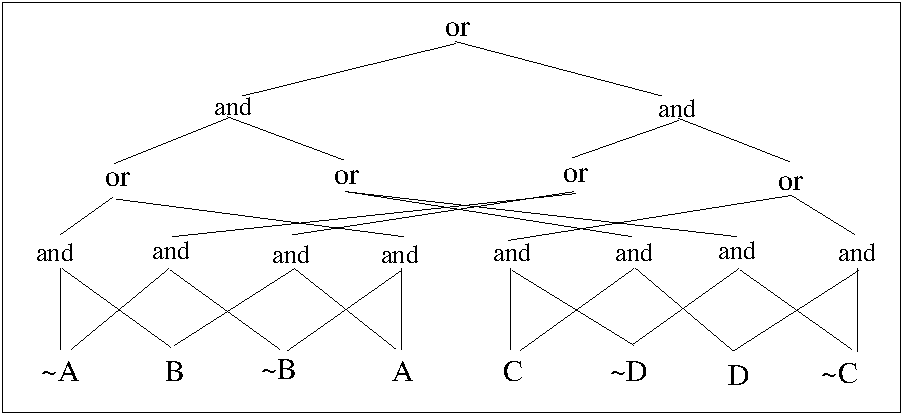
\includegraphics[width=.7\textwidth]{odd}
\caption{A decomposable and deterministic NNF.}
\label{fig:dnnf}
\end{figure}

A Negation Normal Form (NNF) theory is constructed from literals using only conjunctions
and disjunctions \cite{barwise:handbook}, and it can be represented as a directed
acyclic graph in which the leaves are labeled with literals and the internal nodes
are labeled with $\land$ and $\lor$; see Fig.~\ref{fig:dnnf} for an example.
This fragment is universal meaning that for every logical formula there is an
equivalent one in NNF format.
An NNF is said to be decomposable (DNNF) \cite{darwiche:d-dnnfs} if for each conjunction
$\bigwedge_i\phi_i$, the set of variables in each conjunct are pairwise disjoint; i.e,.
$Vars(\phi_i)\cap Vars(\phi_j)=\empty$ for $i\neq j$.
A DNNF supports a number of operations in polytime in the size of its DAG.
For example, we can test whether a DNNF is satisfiable by a single bottom-up pass
over its DAG in linear time.
A DNNF is said to be deterministic (d-DNNF) \cite{darwiche:d-dnnfs} if for each
disjunction $\bigvee_i\phi_i$, the disjuncts are pairwise logically contradictory;
i.e., $\phi_i\land\phi_j\equiv\textbf{false}$ for $i\neq j$.
The NNF in Fig.~\ref{fig:dnnf}, for example, is decomposable and deterministic.
A d-DNNF supports model counting in polytime in the size of its DAG, and model
enumeration in polytime in the size of the output.
Furthermore, given a literal ranking function $r$, one can compute the rank
of the best model in polytime for DNNFs \cite{darwiche:weighted}.

The fragments DNNF and d-DNNF are universal yet translating a CNF theory 
to DNNF format has an exponential cost in the worst case. This translation
is referred to as compilation in the field. There is a publicly available
compiler, called c2d,\footnote{\url{http://reasoning.cs.ucla.edu/c2d}}
that perform this compilation process and that make
use of modern SAT techniques such as conflict-directed backtracking,
clause learning and caching \cite{darwiche:compiler}.
This compiler incurs in the worst case in exponential space in a parameter
called the width of the decomposition tree that is related to the ``connectivity''
of the CNF theory. However, in our experiments, the CNF theories that are
compiled are of low width.

%DNNFs had also been used elsewhere to tackle other combinatorial optimization
%problems such as problems in planning \cite{palacios:icaps05} and diagnosis
%\cite{REF}.

\begin{figure}[t]
\centering
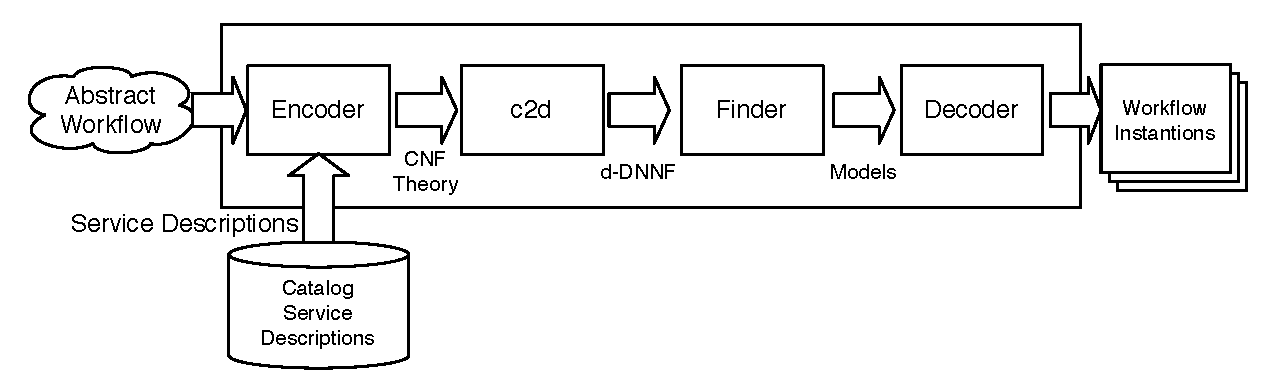
\includegraphics[width=.9\textwidth]{architecture}
\caption{System Architecture}
\label{fig:architecture}
\end{figure}

\section{System Architecture}

We use an architecture that is comprised of a Catalog of service descriptions,
the Encoder, the compiler c2d, the best model Finder, and the Decoder.
Figure~\ref{fig:architecture} depicts the overall architecture of the system.
In this framework, an instance of Workflow Instantiation Problem is defined as an
abstract workflow represented by a conjunctive query on abstract services which
is given as input together with a set set of concrete services defined by views
of abstract services. 

The Catalog is populated with descriptions of abstract and concrete services;
each service is described in terms of input and output attributes, and annotated
with a real value that represents the QoS utility of the service.
The description of the concrete services, that are defined as views of abstract
services, can be generated semi- or automatically using tools such as the DEIMOS
system \cite{AmbiteISWC09}. 

An input instance of WIP is encoded as a CNF theory whose models corresponds to
the instantiations of the workflow by the Encoder. The compiler c2d, an off-the-shelf
component, compiles the CNF formula into d-DNNF.
The Encoder translates the WIP instances into CNF theories, that are then converted
into d-DNNF using c2d. The Finder computes a best model given the QoS parameters
in linear time in the size of the resulting d-DNNF. It is important to remark,
that the compilation process needs to be performed only once as it does not
depend on the value of the QoS parameters. Thus, even if the compilation happens
to be costly in terms of time, this cost can be amortized since the resulting
d-DNNF can be used to find best instantiations with respect to multiple values
of the QoS parameters.
Finally, the Decoder translates the best model returned by the Finder into
a workflow instantiation that solves the WIP.

Given a CNF that encodes a WIP, its d-DNNF is a compact representation of
all the workflow instantiations. That is, one can generate in a backtrack-free
manner all the instantiations of the workflow. If the user is interested in
a best instantiation given the QoS parameters, then it can be computed in
linear time in the size of the d-DNNF. If the user is interested in the 
all the best instantiations, these can be computed in linear time in the
number of them. Finally, if the user is interested in all instantiations,
these can be also computed in linear time in the number of them.
In the latter two cases, if such number is exponential (in the size of the
input), the enumeration of the instantiations is also exponential but
this complexity is intrinsic to the problem and thus cannot be avoided.

In order to make our results more accessible to a general audience, we decided
to present the experimental results in the next section, and leave the formal
and theoretical results for the following section. In this way, the interested
reader may skip the formal details of the approach on a first reading.

\section{Experimental Results}

We conducted an empirical analysis on three benchmarks.
All the experiments were run on a desktop machine with an Intel
Core 2 Duo 2GHz CPU and 4Gb of memory, and the time was measured
with the Unix time command.

The objective of the experiment is to assess the performance
of the proposal on varying conditions. The main benefit of our approach
is that one can compile the logical theory for a problem instance
and then calculate all the instantiations, or the best ones, any 
number of times. The cost model for finding best instantiations
can be changed with no need to recompile the logical theory.
Therefore, the time complexity of our approach is basically the
time to encode the WIP as a CNF plus the time to compile the
CNF into a d-DNNF and the time to decode the models. 
The times to encode and decode are negligible compared to
the time to compile the CNF. Because of this, we focus on the
time to compile the benchmark problems.

The first benchmark consists of problems for air-travel queries.
Concrete services are of the form $V_i(x,y)\qrule\ \flight(x,y,\AL_i)$
where $\AL_i$ is a constant that denotes the name of an airline, 
and $\flight(x,y,\AL_i)$ relates the cities $x$ and $y$ such that
there is a flight between $x$ and $y$ served by $\AL_i$. This concrete
service is assumed to return all flights between two cities with an
specific airline. The workflow has the form 
\[ W(x_1,\ldots,x_n)\ \qrule\ \flight(\PA,x_1,z),\,\flight(x_1,x_2,z),\,\ldots,\,\flight(x_n,\NY,z)\,. \]

\begin{figure}[t]
\centering
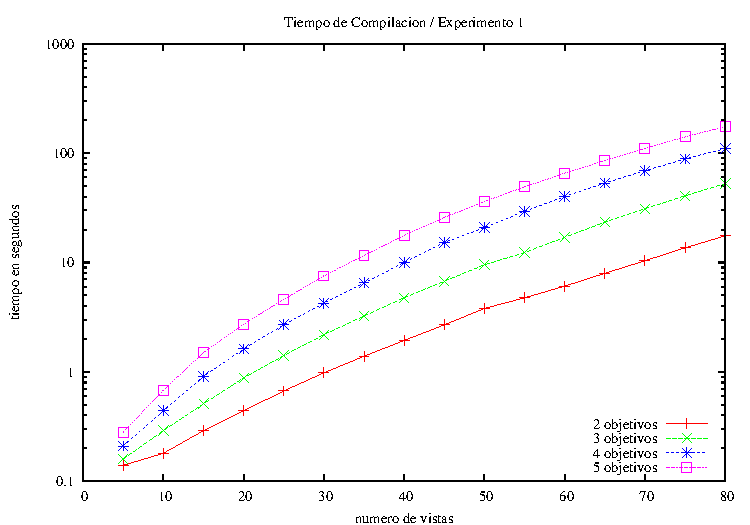
\includegraphics[width=1\textwidth]{plots/plot1}
\caption{Compilation times for experiments I and II for different
number of goals and different number of views. The plots are in
logarithmic scale, and the time is in seconds.}
\label{fig:plot1}
\end{figure}

The benchmark includes instances for workflows with 2 to 5 sub-goals and
sets of 10 to 100 concrete services. The results for the compilation are
shown in panel (a) of Fig.~\ref{fig:plot1}. This is a plot in logarithmic
scale that suggests a sub-exponential behavior. In any case, the results
show good performance since realistic instances of the problem (sets of 100
airlines with 5-stop flights) can be compiled in 328 seconds.
The size in disk of the d-DNNF for 100 airlines and 5-stop flights is 3.4Mb.
On this d-DNNF, the best model can be computed in 0.29 seconds,
and the enumeration of all models in 0.47 seconds.

In an attempt to induce an exponential growth in the compilation time,
in the second benchmark we add a second concrete service for each airline.
This modification increases the number of valid instantiations from linear
to exponential since each leg of a flight can now be instantiated by two
concrete services and thus a flight with $n$ legs may have up to $2^n$
instantiations.
We ran the compiler for instances comprising the same number of workflow
sub-goals and total number of concrete services. The results plotted in
logarithmic scale are shown in panel (b) of Fig.~\ref{fig:plot1}.

These tests show good performance for this type of problems, but they do not
involve concrete services with multiple sub-goals. We therefore designed a
third experiment that consists unstructured, randomly generated instances.
Each instance contains three variables per abstract service, ten distinct
variables and ten distinct constants, six sub-goals in the workflows,
2 to 5 sub-goals in the concrete services, and a varying number of services.
The chance that an argument of an abstract service is bound to a constant is 50\%.
The results are depicted in Fig.~\ref{fig:plot3}.
The compilation time for these instances does not grow monotonically
since they are randomly generated. The same happens for the size of
the theories and the number of models. For example, the d-DNNF for 
a problem with 45 views each with 5 sub-goals is of size 5.1Mb and has
$1.26\times 10^8$ models. The time to find the best model for
this d-DNNF is 0.46 seconds while the time to enumerate all models
is about 17 hours.

\begin{figure}[t]
\centering
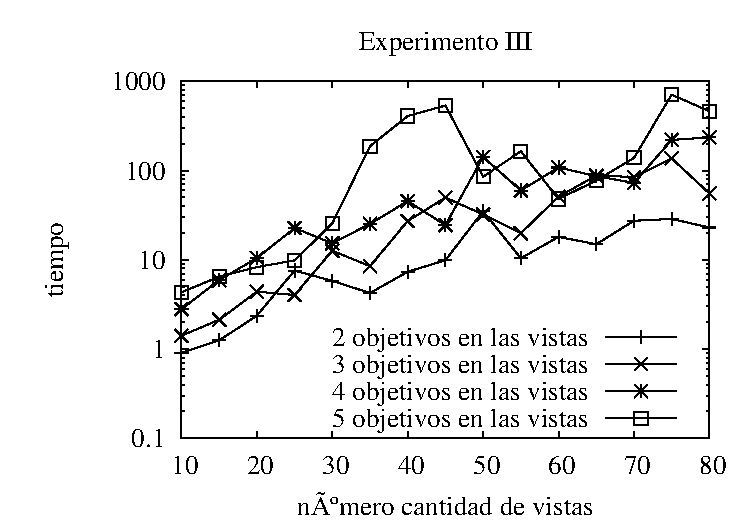
\includegraphics[width=.8\textwidth]{plots/plot3}
\caption{Compilation times for experiments III for different number of goals
and different number of views. The plots are in logarithmic scale, and the time
is in seconds.}
\label{fig:plot3}
\end{figure}

These are preliminary experiments, yet the results show that the
proposed approach efficiently scales for problems with several goals
and views. We believe that these results are encouraging and motivate
us to continue this research. We plan to conduct additional experiments
with other types and sizes of workflows and, when possible, compare with
other approaches.

\section{Formalization}

We consider service catalogs of the form $C=\tup{S,T}$ where $S$ is a set
of predicates that represent abstract services and $T=\{T_s\}_{s\in S}$ is
a collection of tables that represents the result of evaluating the abstract
services. In the context of the WIP, a service catalog $C$ is an idealized
description of the output produced by abstract workflows implemented by
concrete services described as views.
A workflow $W$ over $S$ is a conjunctive query of the form 
\[ W(\vvec{x})\ \qrule\ s_1(\vvec{x}_1),\,s_1(\vvec{x}_2),\,\ldots,\,s_m(\vvec{x}_m)\,, \]
where $s_i\in S$, $\vvec{x}$ is a vector of variables, and each $\vvec{x}_i$
is a vector of variables and constants. The result of $W$ over $C$, denoted
as $W(C)$, is the table with $|\vvec{x}|$ columns that result of the projection
of the relational join $\join\!\!\{T_{s_i}\}_{i=1}^n$ over $\vvec{x}$.
The atoms in the body of $W$ are called the (sub)goals of $W$, and the variables
in the head of $W$ are called distinguished.

A concrete service is described as a view $V$ over $C$ that, following LAV, is
a query over $S$. Given a catalog $C$, a workflow $W$ and a collection of $n$ views
$E=\tup{\{V_i\}_{i=1}^n,\{E_i\}_{i=1}^n}$, we are asked to find all the tuples in $W(C)$
that can be obtained from the views in $E$. That is, we need to find all the
\emph{instantiations}
\[ R(\vvec{x})\ \qrule\ V_{i_1}(\vvec{x}_1),\,V_{i_2}(\vvec{x}_2),\,\ldots,\,V_{i_{m_i}}(\vvec{x}_{m_i}) \]
such that $R(E) \subseteq Q(C)$.
A Workflow Instantiation Problem is a tuple $\tup{S,W,\{V_i\}_i}$ where $S$
is a set of predicates that represent abstract services, $W$ is a workflow over
$S$, and $\{V_i\}_i$ is a collection of views that define the concrete services.
We assume \emph{safe} problems in the sense that all variables mentioned in the
head of the workflow (resp.\ in the head of each view) appear in the body of the
workflow (resp.\ in the body of each view).
Further, we only deal with WIPs with no arithmetic predicates inside the workflow
or views. An instantiation $R$ is \emph{valid} if for all catalogs $C=\tup{S,T}$
and extensions $\{E_i\}_i$, $R(E)\subseteq Q(C)$. A collection $\R$ of valid
instantiations is a solution if for all service catalogs $C=\tup{S,T}$ and
extensions $\{E_i\}_i$, there is no $\R'$ such that $\R(E)\subset\R'(E)\subseteq Q(C)$.

\subsection{Logical Theories}

We use an approach similar to the one described in \cite{arvelo:aaai06} to
encode the WIP. We have limited space to make a comprehensive description of
the logical theory so the reader is referred there for details and formal results.

We identify workflow instantiations by enumerating the models of a logical
theory $\Delta=\Delta_{com}\cup\Delta_{id}^1\cup\cdots\Delta_{id}^N$
where $\Delta_{com}$ specifies how to combine $N$ independent copies theories
$\Delta_{id}$ that cover the goals in $W$.
Each $\Delta^i_{id}$ is a tagged copy $\Delta_{id}$ in which each literal
$\ell$ is tagged as $\ell^i$.
The Instantiation Description (ID) theory $\Delta_{id}$ consists of different
groups of clauses that guarantees that its models are in correspondence with
partial instantiations, while the theory $\Delta_{com}$ contains additional
clauses to guarantee a sound and complete combination of partial instantiations
into a complete instantiation.
The ID theory $\Delta_{id}$ consists of the following variables:
\begin{enumerate}[--]
\item $\{v_0,\ldots,v_n\}$ to indicate which $V_i$ is used, or $v_0$ to indicate the null ID.
\item $\{g_1,\ldots,g_m\}$ to indicate the goals covered by the view.
\item $\{z_{j,k,i}\}$ to indicate that the $j$th goal in $W$ is covered by the $k$th goal in $V_i$.
\item $\{t_{x,y}\}$ to indicate that the variable/constant $x$ in $W$ is mapped into the
      variable/constant $y$ in the view.
\end{enumerate}
The ranges of the indices for the $z$ and $t$ variables depend on the problem.

The following clauses encode the WIP problem in terms of the WIDs.
Rajaraman et al.\ \cite{RajaramanSU95} showed that for queries without negation or
arithmetic comparisons, but with constants, and $m$ goals and $k$ variables in the
head of the workflow, it is enough to consider instantiations of length at most $N=m+k$.
\begin{enumerate}[C10.]
\item[C1.] (At least of view is used): $\bigvee_{i=0}^n v_i$.
\item[C2.] (At most one view is used): $\neg v_i\lor\neg v_j$ for $i\neq j$.
\item[C3.] (Null view equals null): $v_0 \Rightarrow \neg g_j$ for $1\leq j\leq m$.
\item[C4.] (Views are useful): $v_i \Rightarrow \bigvee_{j=1}^m g_j$ for $1\leq i\leq n$.
\item[C5.] (Subgoals covered at most once): $z_{j,k,i} \Rightarrow \neg z_{j,l,i}$ for appropriate $i,j,k,l$.
\item[C6.] (Scope of views): $v_i \Rightarrow \neg g_j$ for goals that cannot be covered by $V_i$.
\item[C7.] (Consistency): $v_i \land g_j \Leftrightarrow \bigvee z_{j,k,i}$ for appropriate $i,j,k$.
\item[C8.] (Dead variables): $v_i \Rightarrow \neg t_{x,y}$ for all $x,y$ with $y\notin V_i$.
\item[C9.] (1-1 for $\exists$ vars): $v_i \land t_{x,y} \Rightarrow \neg t_{x,y'}$ for all
           existential variables $y,y'\in V_i$.
\item[C10.] (Distinguished): $v_i \Rightarrow \neg t_{x,y}$ for distinguished $x$ and existential
            $y\in V_i$.
\item[C11.] (Existential): $v_i\land t_{x,y}\Rightarrow g_j$ for exist.\ $y\in V_i$ and
            goals $g_j$ that contain $x$.
\item[C12.] (Match): $v_i\land z_{j,k,i} \Rightarrow t_{x,y}$ for all $x,y$ that must match
            if $g_j$ is covered by goal $k$ in $V_i$.
\item[C13.] (If all vars in $V_i$ are distinguished, it covers only one goal):
            $v_i \land g_j \Rightarrow \neg g_k$ for appropriate views $v_i$.
\end{enumerate}
These clauses are the same clauses used by \mcdsat\ to encode QRPs \cite{arvelo:aaai06}.
In order to properly manage constant symbols, the clauses must be enhanced with:
\begin{enumerate}[C10.]
\item[C14.] (Direct inconsistency 1): $t_{x,A} \Rightarrow \neg t_{x,B}$.
\item[C15.] (Direct inconsistency 2): $t_{A,x} \Rightarrow \neg t_{B,x}$.
\item[C16.] (Direct inconsistency 3): $\neg t_{A,B}$.
\item[C17.] (Transitivity 1): $v_i\land t_{A,y}\land t_{x,y}\land t_{x,z}\Rightarrow t_{A,z}$.
\item[C18.] (Transitivity 2): $v_i\land t_{y,A}\land t_{y,x}\land t_{z,x}\Rightarrow t_{z,A}$.
\end{enumerate}
Recall that, as shown in Section~2, the main issue when handling
constants is to be sure that not two different constants are mapped
into each other either directly or indirectly.
Clauses C14--C16 prune direct inconsistent mappings, while the last
two clauses implement a restricted propagation of mappings that prune
indirect inconsistencies.
Likewise, the theory $\Delta_{com}$ that specifies how a complete
instantiation contains the following clauses:
\begin{enumerate}[C10.]
\item[C19.] (Cover all goals): $\bigvee_{j=1}^m g^i_j$ for $1\leq i\leq N$.
\item[C20.] (Disjunctive cover): $g^i_k \Rightarrow \neg g^j_k$ for $i\neq j$.
\item[C21.] (Prune symmetries): $g^i_j \Rightarrow \bigvee_{k=1}^{j-1} g^{i-1}_k$
            for $1\leq j\leq m$ and $1\leq i\leq N$.
\item[C22.] (Direct inconsistency 4): $t^i_{x,A} \Rightarrow \neg t^j_{x,B}$.
\end{enumerate}
These clauses provide sound and complete characterization of WIPs in the
sense that their models are in correspondence with the
instantiations of the workflow.

\subsection{QoS Parameters}

For the QoS parameters, we assume a simple additive aggregation model in
which each view $V_i$ is associated with a cost $c(V_i)$ (negative if utility),
and a complete instantiation with the sum of the cost of its views.
An optimal or best instantiation is one with minimum cost, and the
optimal value of the WIP is the cost of an optimal instantiation.
A WIP always has a well-defined optimal value (if there are no instantiations,
its cost is $\infty$), but it may have multiple best instantiations.
The WIP with costs consists in finding all optimal instantiations or
one instantiation, this depends on the particular application.
In our formulation, this can be done from the d-DNNF that encodes $\Delta$
using the literal ranking function $r$ that assigns $r(\ell)=c(V_i)$ if
$\ell=v_i$, and $r(\ell)=0$ if $\ell\notin\{v_1,\ldots,v_n\}$.

\section{Conclusions and Future Work}

We have shown how the propositional theory used in \mcdsat\ for
computing rewritings of queries can be extended to support constants
symbols and thus adapted to the problem of instantiating abstract
workflows. In this work, we adopted a LAV formulation of the
workflow instantiation problem typically found in SOAs.
Our formulation assumes that all concrete services are described
using views over abstract services and that the workflow is 
expressed as a conjunctive queries over the abstract services.
This workflow has resolved all the issues related to the
binding of input and output parameters of services. What
remains is the problem of finding the best instantiation
of the workflow in terms of the QoS parameters.
This formulation of the problem is supported by systems 
like DEIMOS that are able to generate in semi- or
automatic manner LAV descriptions as the one required.

The experimental results show that the approach can be applied to
real-sized workflow problems. The whole approach is only possible
when the compilation of the CNF theory into d-DNNF format succeeds.
In the future, we plan to address this limitation by adapting a
branch-and-bound optimization algorithm that searches the combinatorial
space of instantiations but prunes suboptimal branches with admissible
heuristics.

We also are interested in using other target compilation languages
like Ordered Binary Decision Diagrams.

\bibliographystyle{abbrv}
\bibliography{ref}

\end{document}

